\documentclass{standalone}
\usepackage{tikz}
\usepackage{ctex,siunitx,upgreek}
\usepackage{tkz-euclide}
\usepackage{amsmath}
\usetikzlibrary{patterns, calc}
\usetikzlibrary {decorations.pathmorphing, decorations.pathreplacing, decorations.shapes,}
\begin{document}
\small
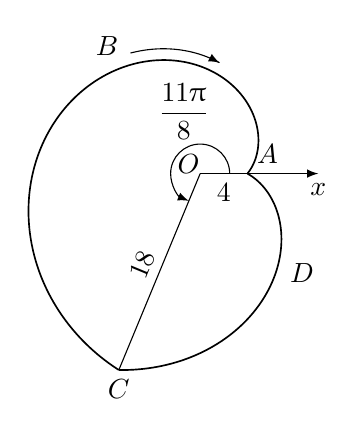
\begin{tikzpicture}[>=latex,scale=0.15]
  \draw[thin,->](0,0)--(10,0)node[below]{$x$};
  \draw[semithick,domain=0:247.5,samples=200] plot (\x:{4+14*\x/247.5});
  \draw[thin,<-,domain=80:120,samples=200] plot (\x:{5+14*\x/247.5});
  \draw[semithick,domain=247.5:360,samples=200] plot (\x:{48.8-22.4*\x/180});
  \node at (2,0)[below]{4};
  \node at (4,0)[above right]{$A$};
  \node at (247.5:18)[below]{$C$};
  \node at (123.75:11)[above left]{$B$};
  \node at (315:9.6)[below right]{$D$};
  \draw(0,0)--(247.5:18)node[midway,sloped,above]{18};
  \draw[->](2.5,0)arc(0:247.5:2.5)node[midway,above]{$\dfrac{11\uppi}{8}$};
  \node at (0,0)[above left,inner sep=0pt]{$O$};
\end{tikzpicture}
\end{document}